%%==================================================%%
%% Last Modified: Wed Jan 10 20:22:53 2007.
%%==================================================%%

%% For CSE.UNSW Technical Report
\documentclass[titlepage]{csetr-notr}

\usepackage{graphicx}
\usepackage{amsmath,amsfonts,amsthm,amssymb}
\usepackage{setspace}
\usepackage{url}
\usepackage{fancyhdr}
\usepackage{lastpage}
\usepackage[font={small,it},belowskip=-10pt,aboveskip=5pt]{caption}
\usepackage{multicol}
\usepackage{subfigure}
\usepackage{color}
\usepackage{framed}
\usepackage{tabularx}

%\usepackage{float}
%\usepackage{extramarks}
%\usepackage{chngpage}
%\usepackage{soul,color}
%\usepackage{graphicx,float,wrapfig}
\definecolor{shadecolor}{rgb}{1,1,0}

\renewcommand{\and}{\hspace{.5cm}}
\newcommand{\zz}{\hspace{.5cm}}

%% specify the TR number and date
\trnumber{0701}
\trdate{\reportDate}

\newcommand{\SupervisorName}{Dr. Xiongcai Cai}
\newcommand{\StudentName}{Shaobo\ Dang}
\newcommand{\StudentID}{3384106}
\newcommand{\StudentEmail}{sdang@cse.unsw.edu.au}
\newcommand{\reportDate}{\today}
\newcommand{\researchTitle}{Thesis Proposal \\ \vspace{.8in}\textbf{Bayesian Nonparametric Model in Active Learning}}
\newcommand{\assignmentTitle}{ Research Proposal}

\title{%
  \researchTitle
}
\author{%
  \StudentName\ (\StudentID)\\%[2em]
  \email{\StudentEmail}
}


\date{}
\pagestyle{fancy}
% Setup the header and footer
\pagestyle{fancy}
\lhead{\StudentName}
\chead{}
\rhead{\assignmentTitle}
\lfoot{\reportDate}
\cfoot{}
\rfoot{Page\ \thepage\ of\ \pageref{LastPage}}
\renewcommand\headrulewidth{0.4pt}
\renewcommand\footrulewidth{0.4pt}

\fancypagestyle{plain}{
    \fancyhf{} %clear all header and footer fields on pagestyle plain for chapter titles
    \lhead{\StudentName}
    \chead{}
    \rhead{\assignmentTitle}
    \lfoot{\reportDate}
    \cfoot{}
    \rfoot{Page\ \thepage\ of\ \pageref{LastPage}}
    \renewcommand\headrulewidth{0.4pt}
    \renewcommand\footrulewidth{0.4pt}
}

\setcounter{tocdepth}{4}
\setcounter{secnumdepth}{4}
\let\stdsection\section
\renewcommand\section{\newpage\stdsection}

%%%%%%%%%%%%%%%%%%%%%%%%%%%%%%%%%%%%%%%%%%%%%%%%%%%%%%%%%%%%%

\begin{document}
\begin{spacing}{1.2}
\maketitle

\setcounter{page}{2}

\tableofcontents

\section{Introduction}
%bigdata
\indent Data Mining has been an heating area in Machine Learning. It is especially important in the information age since the seemingly meaningless data often containing potential opportunity, as can be seen from large Internet companies such as Google, Facebook and Amazon \cite{mcafee2012big}on their investment on large data processing project. 

The primary task in data mining is to find the underlying distribution that generates the observed data to guide the computer to process the similar data automatically, saving the cost of both time and expense. As the data often consists of multi-modal distribution, modeling the distribution as a mixture of simpler distribution is found to be a well approximation. In parametric settings, the number of sub-distribution is fixed value which may cause the model fail to funtion as the complexity is not synchronized that of the data. Instead, Bayesian Nonparametric model, especially the Dirichlet Process employs a infinite countably number of components to handle the analysis by placing a prior distribution for mixing distribution. The nature of this set of problem bypasses the need to "determine" the number of comopnents in a finite mixture model. 

Though a very promising and relatively simpler way to model, it is often difficult to process the following inference which is the main part of analysis. Except for placing conjugate prior, the desirable posterior distribution of most non-conjugate prior model is hard to obtain. 

Use of Dirichlet process mixture models has been computationally feasible with the development of Markov Chian Monte Carlo methods for sampling from the posterior distribution of the parameters of the component distritution given observed data. But there need more research work on addressing the slow convergency problem. Though conjugate prior is preferable for it allows to introduce Gibbs sampling methods, it narrows the generalization of Dirichlet Process to address more complicated problem. In most cases, the non-conjugate prior is placed, thus it should be researched on how to use MCMC under such circumstances. Also research on applications based on DPMM that requires fast convergency will be conducted.

 




\section{Aim Of Research}\label{aor}
\hyphenation{Non-para-metric}
The primary objective of this research is to introduce the Bayesian Nonparametric(BNP) theory to the general framework of Active Leaning. We aim to design a new learning framework enabling the growing of model complexity without a great compromising in accuracy and a growth in cost.
\colorbox{green}{The}initial motivation is take advantages of the merits , as for active learning the efficiency and for BNP the flexibility, to make up for their disadvantage, as for active learning low sampling procedure and and for BNP low convergency rate\cite{gershman2012tutorial,escobar1995bayesian,Settles2010}. In this proposal, we will exploit the general problems in this two distinct areas and the  potential performance when combined together.  The main aims of this research consist of the following parts(will be in addressed in detail in later part) 
\begin{enumerate}
\item{\textbf{Develop a new sampling methods in active learning}}\\
 Sampling strategy lies in the core of active learning scheme. Most approaches select either informative or representative unlabeled instances. But it is usually challenging to find the querying instances that are both informative and representative. Thus in this research, a new approach is to be proposed to provide a systematic way to select samples having both features, and the effectiveness will be validated.
\item{\textbf{Combining BNP learning theory with active learning theory  }}\\

 Bayesian Nonparametric(BNP) model is very promising in development recent machine learning theory. Every classical learning could be reinterpreted under context of BNP, ranging from classification, regression to density estimation. Another flexibility of it is that the complexity of model is adaptive to the size of the learning problem, making it easier to generalize. We are aiming to take these advantages and introduce them into the active learning theory and exploit the performance of the framework.  
\end{enumerate}


\section{Literature Review}
This section summarizes the overview of the two main topics of this research. The first part is the general introduction to active learning and current work on this topic, followed by the review on bayesioan nonparametric models sharing the same structure. 
\newcommand{\argmax}[1]{\underset{#1}{\operatorname{arg}\,\operatorname{max}}\;}
\newcommand{\argmin}[1]{\underset{#1}{\operatorname{arg}\,\operatorname{min}}\;}
\subsection{Background}
Large Data sets are often heterogeneous, cased b amalgams from underlying sub-populations. When doing analysis on such data sets, it often involves grouping the data to make the original data more heterogeneous. Traditionally, parametric models using a fixed and finite number of parameters could be used, but they suffer from over- or under-fitting of data when there is a misfit between the complexity of the model and the amount of data available. Thus, model complexity selection is often an important issue in parametric modeling. But whether we use cross validation or marginal probabilities as the basis for selection, model selection is an operation that is fraught with difficulties, especially when the data set grows larger and larger. 

The Bayesian Nonparametric approach is an alternative to parametric modeling and selection. Under this scheme, the model comes with an unbounded complexity, and under-fitting and over-fitting are mitigated. Typically, we assume that the observed data set $x_1,x_2,\cdots,x_i$ are i.i.d(Independent Identical Distributed) sampled from some underlying unknown distribution $\mathbb{F}$. In Bayesian approach,  a prior is placed over $\mathbb{F}$ then he posterior over  $\mathbb{F}$ given data is computed. This prior over distributions is given by a parametric family. But constraining distributions to lie within parametric families limits the scope and type of inferences that can be made. Instead, the nonparametric approach used a prior over distributions with wide support, typically the support being the space of all distributions.  The Dirichlet Process is currently one of the most popular Bayesian Nonparametric Models. It was first formalized in [1] for general Bayesian statistical modeling.,as a prior over distributions with wide support yet tractable posteriors. But the Dirichlet Process is limited by the fact that draws from it are often discrete distributions, and tractable posterior is hard to obtian when it generalized to more general non-conjugate priors until MCMC techniques became available in the area. 
\subsection{Dirichlet Process}
\subsubsection{Dirichlet Distribution}
A Dirichlet distribution is defined on the $\mathit{(k-1)}$-dimensional probability simplex, whic is a surface in $\mathbb{R}^k$ denoted by $\Delta_k
$ and defined to be the set of vectors whose $k$ components are non-negative and sum to 1, that is
\begin{equation}
\Delta_k=\{q\in \mathbb{R}^k|\sum\nolimits_{i=1}^{k}q_i=1,q_i\geq 0\ for\ i=1,2,\cdots,k\}
\end{equation}
While the set $\Delta_k$ lies in a $k$-dimensional space, $\Delta_k$ is itself a $(k-1)$-dimensional object. Each point $q$ in the simplex can be thought of as a probability mass function(pmf) in its own right. The Dirichlet distribution can be thought of as a probability distribution over the $k-1$-dimensional probability simplex $\Delta_k$; that is, as a distribution over pmfs of length $k$.


\textbf{Dirichlet Distribution}: Let $Q=[Q_1,Q_2,\cdots,Q_k]$ be a random pmf, i.e. $Q_i\geq 0$ for $i=1,2,\cdots,k$ and $\sum\nolimits_{i=1}{k}Q_i=1$. In addition, suppose that $\alpha=[\alpha_1,\alpha_2,\cdots,\alpha_k]$ with $\alpha_i>0$ for each $i$, and let $\alpha_0=\sum\nolimits_{i=1^k\alpha_i}$. Then $Q$ is said to have a Dirichlet distribution with parameter $\alpha$, which we denote by $Q\sim Dir(\alpha)$, if it has $f(a;\alpha)=0$ then $q$ is not a pmf, else if $q$ is a pmf then
\begin{equation}
f(q;\alpha)=\frac{\Gamma(\alpha_0)}{\prod\nolimits_{i=1}^{k}\Gamma(\alpha_i)}\prod_{i=1}^{k}q_i^{\alpha_i-1}
\end{equation}
where $\Gamma(s)$ denotes the gamma function, a generalization of the factorial function, for $s>0, \Gamma(s+1)=s\Gamma(s)$, and for positive integers $n$, $\Gamma(n)=(n-1)!, \Gamma(1)=1$. 
\begin{figure}[tbph!]
	\centering
	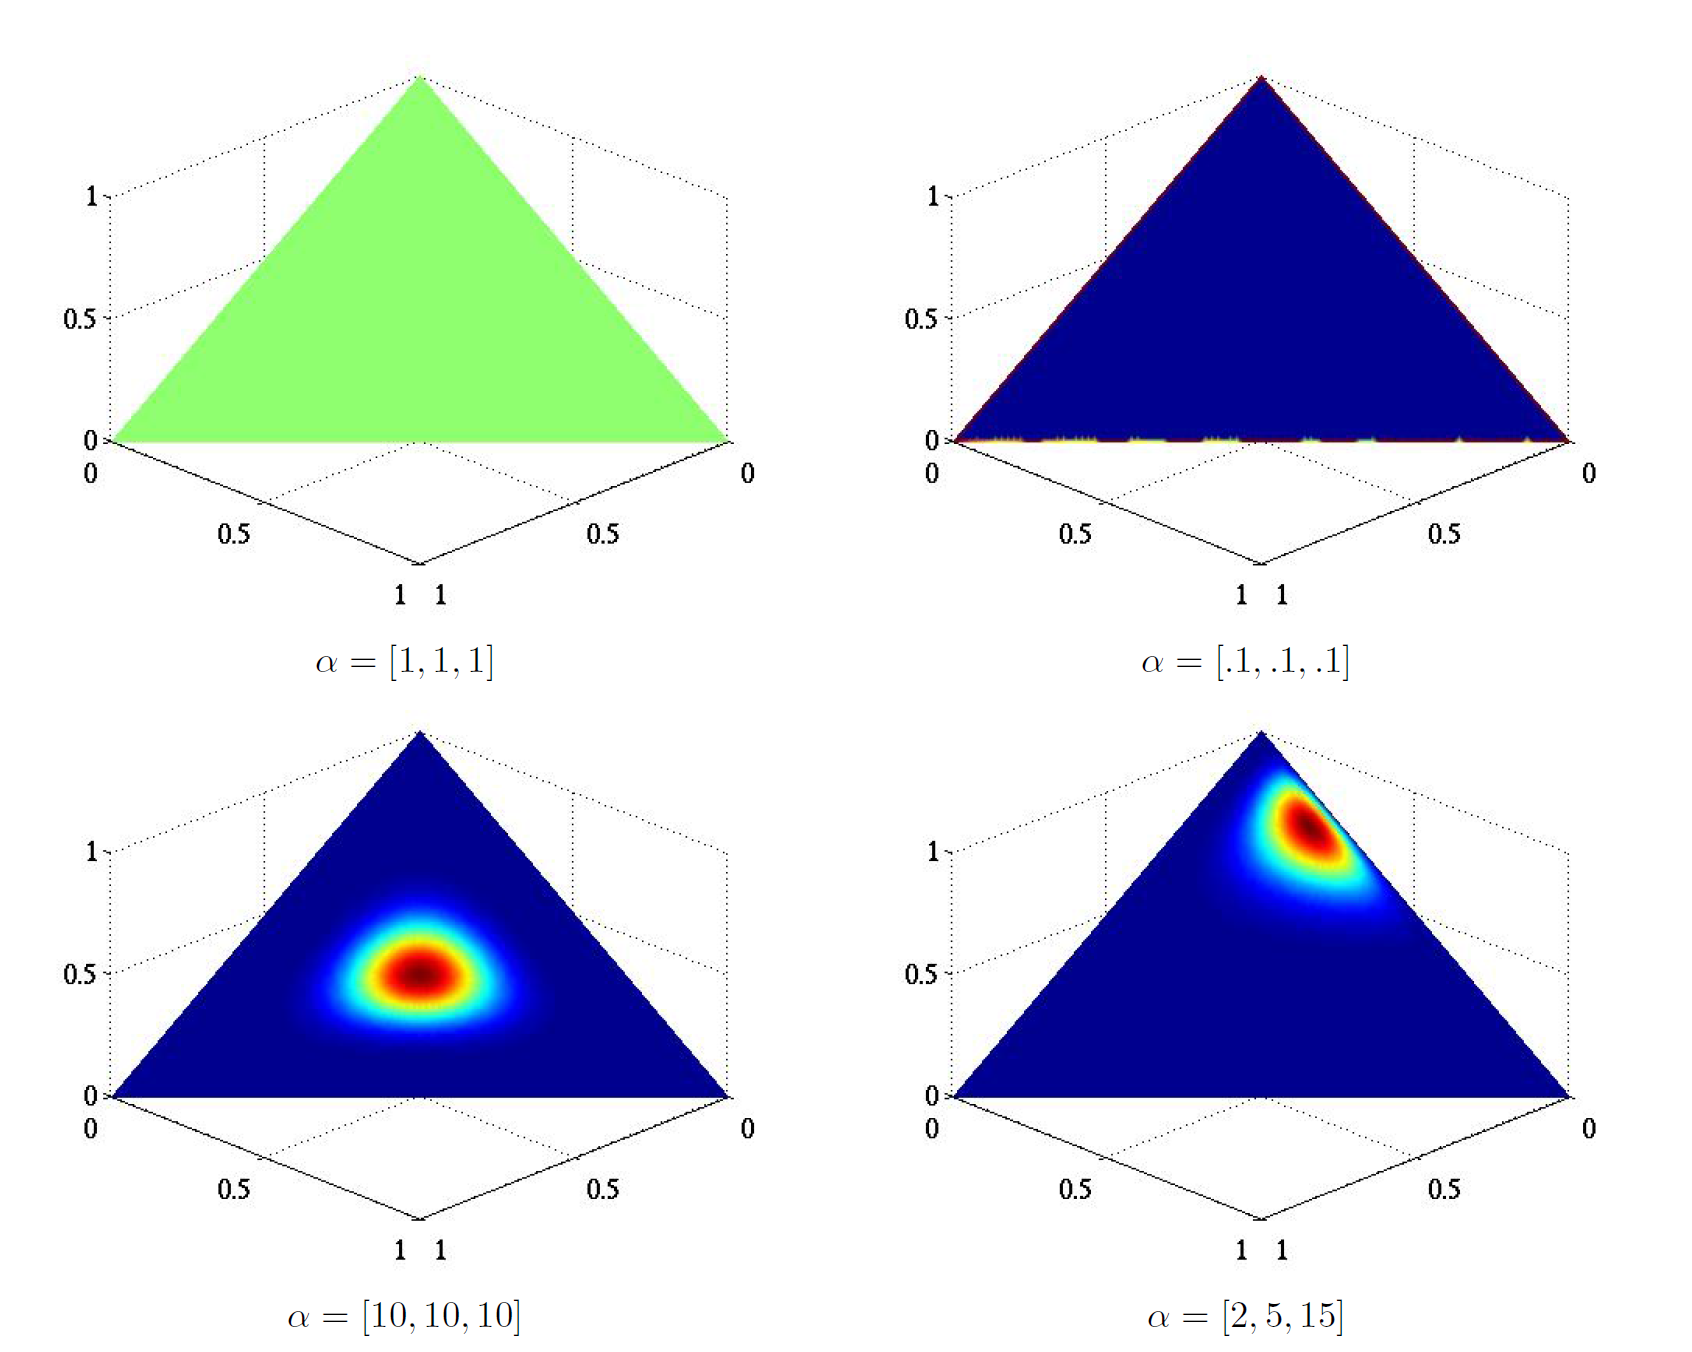
\includegraphics[width=\linewidth]{DirDis}
	\caption{Dirichlet distribution density plots(blue=low, red=high) over the probability simplex in $\mathbb{R}^3$ for various values of the parameter $\alpha$}
	\label{fig:DirDis}
\end{figure}
Fig. \ref{fig:DirDis} shows the plots of the density fo the Dirichlet distribution over the two-dimensional probability simplex for $k=3$ events lying in three-dimensional Euclidean space over a variety of parameter vector $\alpha$. When $\alpha=[1,1,1]$, the Dirichlet distribution reduces to uniform distribution over the simplex. When all the components of $\alpha$ satisfy $\alpha_i>1$, the density is monomodal with its mode somewhere in the interior of the simplex. And when $\alpha_i<1$, the plots has sharp peaks at the vertices of the simplex. Another important feature should be mentioned, as can be seen from the definition of Dirichlet distribution, is that the support is open thus does not include the vertices or edge of the simplex, which in reality means that no component of a pmf drawn from a Dirichlet will ever be zero.  Fig. \ref{fig:DPsample} shows plots of samples drawn i.i.d from different Dirichlet distributions.

\begin{figure}[tbph!]
	\centering
	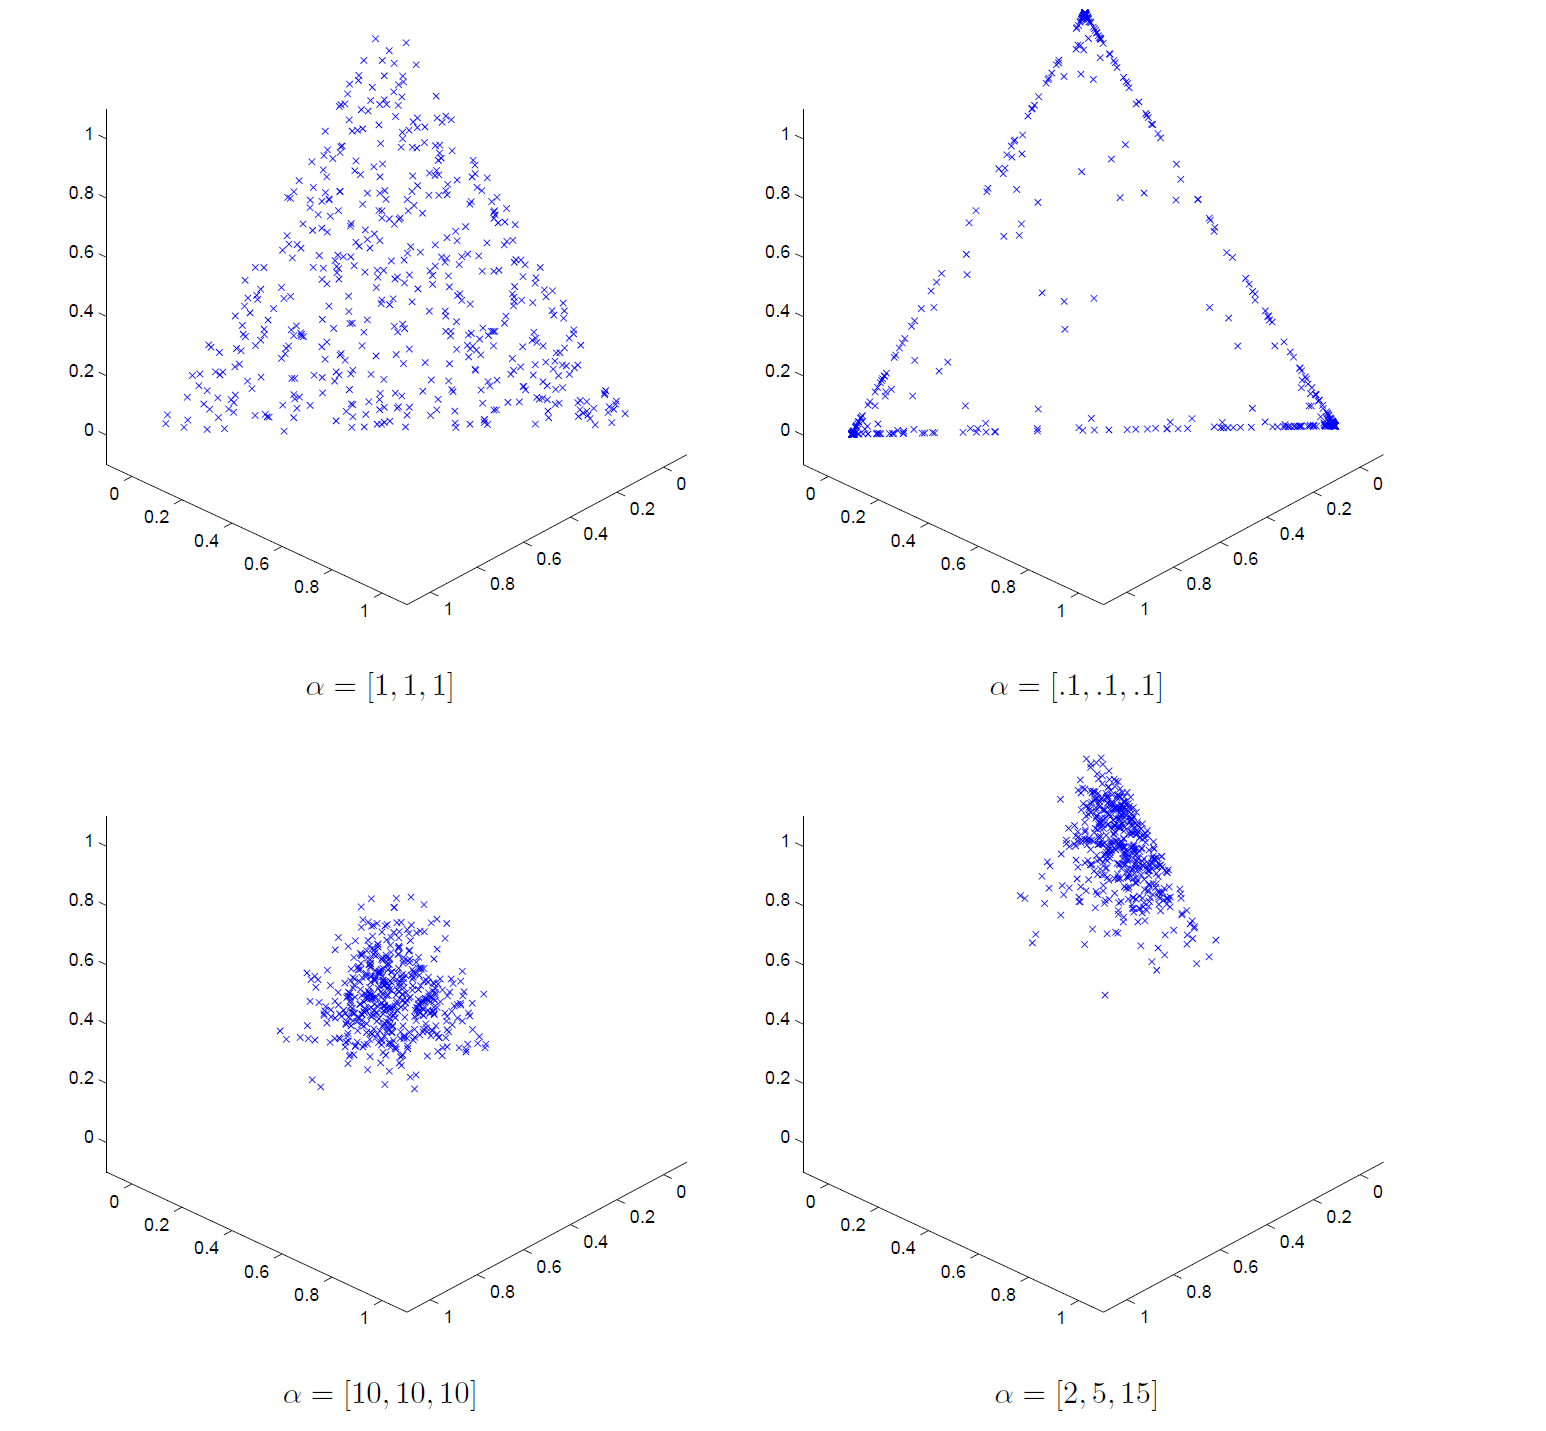
\includegraphics[width=\linewidth]{DPsample}
	\caption{Plots of sample pmfs drawn from Dirichlet distributions over the probability simplex in $\mathbb{R}^3$ for various values of parameter $\alpha$}
	\label{fig:DPsample}
\end{figure}
\subsubsection{Dirichlet Process}
A Dirichlet Process is a distribution over probability distributions. Suppose that $\mathit{G}$ is a probability distribution over a measurable space $\Theta$, then  $\mathit{G}$ is a probability distribution over $\Theta$ and a DP is a distribution over all such distributions. A DP is parameterized b a concentration parameter $\alpha$ and a base measure(base distribution) $\mathit{H}$. So, the formal definition of a DP would be
\begin{equation}
G\sim  DP(\alpha,\mathit{H})
\end{equation}
it means for a finite set of measurable paritions $A_1\cup\cdots\cup A_k=\Theta$, 
\begin{equation}
(G(A_1)\cdots,G(A_k))\sim Dir(\alpha H(A_1),\cdots,\alpha H(A_k))
\end{equation}
which means the probabilities that  $\mathit{G}$ assigns to any finite
partition of  $\Theta$ follow a Dirichlet distribution  with parameters
$(\alpha H(A_1),\cdots,\alpha H(A_k))$.

Since $G$ is a random distribution we can inturn draw samples from $G$ itself. Let $\theta_1,\theta_2,\cdots,\theta_n$ be a sequence of independent draws from $G$. What is the posterior distribution of $G$ given observed values of $\theta_1,\theta_2,\cdots,\theta_n$. In other words, what is the posterior predictive distribution for a new item $p(\theta_{N+1}|\theta_1,\theta_2,\cdots,\theta_n)=\int p(\theta_{N+1}|G)p(G|\theta_1,\theta_2,\cdots,\theta_n)dG$? It is shown in ... that 
\begin{equation}
	(G(A_1),\cdots,G(A_k))|(\theta_1,\theta_2,\cdots,\theta_n)\sim Dir((\alpha H(A_1)+n_1,\cdots,\alpha H(A_k)+n_k)
\end{equation}
where $n_k=\#\{i:\theta_i\in A_k\}$ is the number of observed values in $A_k$. Rewriting the posterior DP, we have:
\begin{equation}
G|(\theta_1,\theta_2,\cdots,\theta_n)\sim DP(\alpha+n,\frac{\alpha}{\alpha+n}H+\frac{n}{\alpha+n}\frac{\sum\nolimits_{i=1}^{n}\delta(\theta_i)}{n})
\end{equation}
and for the posterior distribution,
\begin{equation}
\begin{split}
p(\theta_{N+1}|\theta_1,\theta_2,\cdots,\theta_n)&= E[G(A)|\theta_1,\theta_2,\cdots,\theta_n] \\
&=\frac{1}{\alpha+n}\left(\alpha H+\sum\limits_{i=1}^{n}\delta_{\theta_i}\right)
\end{split}\label{eqa:dppos}
\end{equation}
Therefore the posterior base distribution given $\theta_1,\theta_2,\cdots,\theta_n$ is also the predictive distribution of $\theta_{n+1}$. The sequence of predictive distribution \ref{eqa:dppos} for $\theta_1,\theta_2,\cdots,\theta_n$ is very important and different interpretations on it indicate different properties of the result. To better understand it, we will introduce the most famous three representations of \ref{eqa:dppos}: \textbf{P\'{o}lya urn, Chinese Restaurant Process, Stick-breaking Process}.
\begin{itemize}
	\item \textbf{P\'{o}lya urn} \\
	In this analogy, suppose we are drawing colored balls from an urn, $\theta_i$ represents the color of the $i$-th ball drawn . For each ball drawn, we place it back  and add another one in the same color into the urn. In  the beginning, we pick a color drawn from $H$, paint a ball with that color and drop it into the urn. In the following $n$th step, we will either, pick a new color with probability$\frac{\alpha}{\alpha+n}$, or with probability $\frac{n}{\alpha+n}$ pick a random ball out of the urn.  This process induces a "rich get richer" property on the frequencies of colors inside the urn. Also, it should be noticed that the predictive distribution has point masses located at the previous draws  $\theta_1,\theta_2,\cdots,\theta_n$. Thus the distribution $G$ itself has point masses. When sample size grows larger, the value of any draw will be repeated by another draw, implying that $G$ is composed only of a weighted sum of point masses and thus  it is a discrete distribution.
	\item \textbf{Chinese Restaurant Process}\\
	Another representation of Dirichlet Process-Chinese Restaurant Process(CRP) implies a clustering property. Equation \ref{eqa:dppos} could be rewrite as :
	\begin{equation}
		p(\theta_{N+1}|\theta_1,\theta_2,\cdots,\theta_n) = \frac{1}{\alpha+n}\left(\alpha H+\sum\limits_{i=1}^{n}n_k\delta_{\theta_i^\star}\right)
	\end{equation}
	where $\theta_i^\star$ is the unique values among $\theta_1,\theta_2,\cdots,\theta_n$, and $n_k$ is the number of repeats of $\theta_i^\star$. $\theta_i^\star$ will be repeated by $\theta_{n+1}$ with probability proportional to $n_k$. The larger $n_k$ is, the hight the probability that it will grow. This is similar to the "rich get richer" scheme in \textbf{P\'{o}lya urn}, where large clusters grow larger. We can see that the unique values  of $\theta_1,\theta_2,\cdots,\theta_n$ induce a partitioning of the set $[n]=\{1,2,\cdots,n\}$ into clusters such that within some cluster $k$, the $\theta_i$'s take on the same value $\theta_k^\star$. The random partion encapsulates all the properties of the DP. If we invert the generative process, we can reconstruct the joint distribution over $\theta_1,\theta_2,\cdots,\theta_n$ by first drawin ga random partion on $[n]$, then each cluster $k$in the partition draw a $\theta_k^\star\sim H$, and finally assign $\theta_i=\theta_k^\star$ for each $i$ in cluster $k$. 
	
	The distribution over partitions is called the Chinese Restaurant Process(CRP) in which we have a Chinese restaurant with infinite tables, each of which can seat an infinite number of customers. The first customer enters the restaurant and sits at the first table. And in the following, when the $n+1$th customer comes, he will either joins a tale $k$ with probability propotional to the number $n_k$ of people already sitting there or sts at a new table with probability propotional to $\alpha$. The CRP define a distribution over partitions of $[n]$ and a distribution over permutations of $[n]$. 
	\item \textbf{Stick-breaking Construction} 
	The  third representation of DP is very intuitive and the most widely used one to generate a sample from it. By knowing the fact that draws from a DP consists actually of a weighted sum of point masses, ...provides a constructive and straightforward definition of the DP. It simply following the flowwin steps.
\begin{eqnarray}
	\beta_k\sim Beta(1,\alpha)&\quad&\theta_k^\star\sim H,\\
	\pi_k=\beta_k\prod_{l=1}^{k-1}(1-\beta_k)&\quad&G=\sum_{k=1}^{\infty}\pi_k\delta_k^\star,\\
\end{eqnarray}
Then we have $G\sim DP(\alpha,H)$. The construction of $\pi$ could be interpreted as breaking a stick of length 1 step by step. First break it at $\beta_1$, assigning $\pi_1$ to be the length of segment we just got. Then recursively breaking the remaining portion to obtain $\pi_2,\pi_3,\cdots,\pi_{n-1}$. THis is a very straightforward and simple procedure.
\end{itemize}   

\subsubsection{ Dirichlet Process Mixture Models}\label{bnp}
In this section, we will briefly describe the Dirichlet Process Mixture Model
Most machine learning problem is targeted to learn a set of parameters describing the model from training data set. This sort of learning is often evaluated in two terms, with the first one being how well the model fits the data, expressed as accuracy or squared error, and the second one being a complexity penalty(favoring simpler models)\cite{gershman2012tutorial,escobar1995bayesian}, also referred to as Ocam's Razor. In practical problem, the model complexity is hard to evaluate. Improper model complexity will lead to over-fitting or under-fitting\cite{gershman2012tutorial,muller2004nonparametric}, which will then affect the model generalization, i.e to be applied to practical use. Although through rigid training, desirable models could be trained but this is basically a trial and error process\cite{hjort2010bayesian}. That is the movivation of discovering adaptive model complexity selection methods, among which Bayesian Nonparametric Method is the most widely used.

DP, as the most widely used methods among Bayesian Nonparametric Models, has found applications in  both statistics and machine learning, including Bayesian model validation, density estimation and clustering via  mixture models, among which the last one is the most salient  when talking about DP. 

Model validation is to evaluate whether a model gives a good fit to observed data. Under Bayesian approach, we would usually compute the marginal probability of the data under  the model  and compare the  marginal probability to that of other candidate model. The one with the highest probability will be chosen as the best fitting to the observed data. Here arises an issue that how to choose the models to be compared. Usually, a set of candidate models as large as possible would be desirable. But it would be easier if we re-think this in a Bayesian Nonparametric way, i.e. to use the space of all possible distribution as our comparison class, with a prior over distributions. The DP is always the first priority for its similar nature to this problem. The approach is to use the given parametric model as the base distribution of the DP, with DP serving as a nonparametric relaxation around this parametric model. If the parametric model performs as well or better than the DP relaxed model, we are convinced that the model is valid.

For density estimation, the aim is to modeling the latent density from which the observed data is drawn. To avoid the poor performance caused by the limitation in parametric model, we again employ a Nonparametric prior over all densities. If we drawn samples from a DP, which is  distribution over distribution, we will obtain a random distribution which is discrete,thus has no densities. The solution is to smooth out draws form the DP with a kernel. Let $G\sim DP(\alpha,H)$ and $f(x|\theta)$ be a family of densities indexed by $\theta$. Then 
\begin{equation}
p(x)=\int f(x|\theta)G(\theta)d\theta
\end{equation}

The most common application of the Dirichlet process is to cluster data using mixture  models. The traditional finite mixture model assumes that there are $K$ clusters, each associated with a parameter $\theta_k$. Each observation $y_n$ is assumed to be generated by first  choosing a sluster $c_n$ according to $P(c_n)$ and then generating the observation from its corresponding observation destribution parameterized by $\theta_{c_n}$. Finite model can accomodate many kinds of data by changing the data generating distribution.

Bayesian mixture models further contain a prior over the mixing distributions. The nature of Dirichlet process will translate the mixing model to a countably infinite number of components. we model a set of observations $\{x_1,\cdots,x_n\}$ using a set of latent parameters  $\{\theta_1,\cdots,\theta_n\}$, each $\theta_i$ is drawn I.I.d from $G$, while each $x_i$ has distribution $F(\theta_i)$ parameterized by $\theta_i$:
\begin{eqnarray}
x_i|\theta_i&\sim& F(\theta_i)\\
\theta_i|G&\sim& G\\
G|\alpha,H&\sim& DP(\alpha,H)
\end{eqnarray}\label{eqa:DPM}
Because $G$ is discrete, multiple $\theta_i$'s can take on the same value simultaneously, and the model above can be seen as a mixture model, where $x_i$'s with the same value of $\theta_i$ belong to the same cluster. The mixture perspective can be made more in agreement with the usual representation of mixture models using the stick-breaking construction. Let $z_i$ be a cluster assignment variable, which takes on value $k$ with probability $\pi_k$. Then equation \ref{eqa:DPM} could be expressed as:
\begin{eqnarray}
\pi|\alpha\sim GEM(\alpha)& \quad &\theta_k^\star|H\sim H \\
z_i|\pi\sim  Mult(\pi)& \quad & x_i|z_i,\{\theta_k^\star\} \sim F(\theta_{z_i}^\star)
\end{eqnarray}
with $G=\sum\nolimits_{k=1}^\infty\pi_k\delta_{\theta_k^\star}$,  $\theta_i=\theta_{z_i}^\star$, $\pi$ being the mixing proportion, $\theta_k^\star$ being the cluster parameters, $F(\theta_k^\star)$ being the distribution over data in cluster $k$ and $H$ the prior over cluster parameters.

From above expression, it is seen that DP mixture model is an infinite mixture model-a mixture model with a countably infinite number of clusters. Different from finite mixture model using a fixed number of clusters, $\pi_k$'s decrease exponentially quickly, and only a small number of clusters will be used to model the data a priori. In the DP mixture model, the actual number of clusters used to model data is not fixed, and can be automatically inferred from data using the usual Bayesian posterior inference framework. The equivalent operation for finite mixture models would be model averaging or model selection for the appropriate number of components.
\begin{tabular}{|c|c|c|}
	\hline \rule[-2ex]{0pt}{5.5ex}  & \textbf{Indexing}& \textbf{Partition Labels} \\ 
	\hline \rule[-2ex]{0pt}{5.5ex}  \textbf{P\'{o}lya Urn & sequence of draws of balls  & ball colors  \\ 
	\hline \rule[-2ex]{0pt}{5.5ex} \textbf{Chinese Restaurant Process} & sequence of incoming customers &  different dishes\\ 
	\hline \rule[-2ex]{0pt}{5.5ex}  \textbf{Clustering}&sequence of the natural numbers  & clusters \\ 
	\hline 
\end{tabular} 
\subsection{Inference}



\subsection{Summary}

In this section, we briefly review the two main topic in this proposed research. Generally, Active Learning is an important subsection in machine learning and very promising since it aims to address the bottleneck due to insufficient training instances. We exploited the general problem and main aspects in active learning. And for Bayesian Nonparametric models, it tries to overcome the shortcomings in traditional parametric methods and the flexibility allows for adaption of the model to fit the data,  this is especially important on the model generalization. 

By the analysis in this section, these two branches could be complementary to each other if these are used under the same famework and form a loop of feedback for each other's training stage. BNP model will cluster the dataset adaptively and recommend the most representative sample for active learning. Similarly, active learning will in returen recommend the BNP model which set of point is more preferred which will guide the BNP model updating. 

This close-loop framework is the one we are desired to develop, the performance of similar frameworks in the other area has been proved\cite{zhang2011close}.
\section{Methodology}

This section will describe the methodology to fulfill the research target. As mentioned in the \ref{aor}, the primary goal of this research is to introduce the bayesian learning method into active learning framework to handling the learning problem with variant size of data set and enable the model flexible enough to adapt the model complexity. 
\begin{figure}[htbp]
\centering
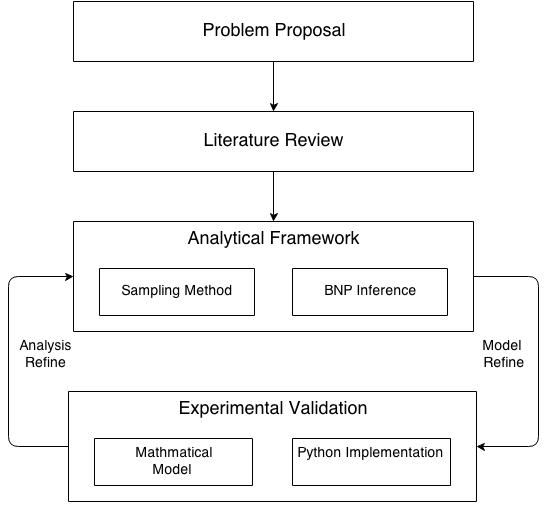
\includegraphics[width=\linewidth]{proposal}
\caption{Research Flowchart}
\label{fig:proposal}
\end{figure}

Fig\ref{fig:proposal} is the main flowchart.  briefing the detailed process, and in each main stage the major work should be:
\begin{enumerate}
 \item \textbf{Literature Review}
 
 This part should not be restricted just to the two main mentioned topics, instead during this procedure, a comprehensive review on the machine learning literature should be carried out. Besides the classical learning theories, extensive reading on analysis of their characteristics and application should also be focused on. The goal is to gain a general understanding of the theory framework, relation to other learning theory,  their history, development and current research. 
 
 \item \textbf{Develop a new sampling method in active learning}
 
 Currently, the general querying mehtods in active learning is to select either informative or representative unlabeled instances\cite{huang2010active}. It remains a challenge to select instances that are distinct on both features\cite{huang2010active}. Informativeness is the measurement of a instance on the prediction ability on the labeled data while the representativeness is the prediction ability on the unlabeled data. The current popular approaches such as query-by-committee\cite{Settles2010}, uncertainty sampling\cite{Settles2010} and so on are all under the framework of querying informative instances. The performance is greatly improved when compared to the algorithms without the active learning procedure. But all these approaches is unable to exploit the potential abundance in the unlabeled data set. Thus the aim of the research is to try to improve the efficiency by diving into the unlabeled data set while maintaining the performance on labeled dataset. This requries the sampling procedure should take into consideration both the informativeness and representativeness of an instance. Thus the new sampling method should be in the form of measuring the desired sample's representative ability in unlabeled data set and its informativeness on the change of model. We will dive into the theoretical analysis on the current different sampling scheme and try to combine them under the same framework. The effectiness of the proposed framework will be tested through experiment and the performance will be used for analysis refine.
 
 \item \textbf{Research on Bayesian Non-parametric Learning scheme}
 
 As the second main research topic, it is also very important to develop the overall learning scheme. BNP model, although very flexible and covering multiple learning tasks. The main focus on this area is how to overcome the low convergency rate in traditional BNP learning. Derived from traditional nonparametric model, Bayesian Non-parametric method is also constrained by the common shortcoming of nonparametric family, which is the high cost on resources\cite{ghosh1982nonparametric,vapnik1998statistical}. Every sample should be kept for the model updating, which will be a disaster as dimension of data set grows. In this research, we aim to bring active learning procedure into the BNP model. During the model updating, instead of storing all training samples, only those is most representative and informative will be kept. The key problem is how to make most of the selected samples in BNP learning process as all the parameters will be updated by using them.  
 \item \textbf{Implementation and Experiment}
 
 This steps include implementing the proposed framework and test the algorithm on different data set regarding the specific problem this framework will be used to evaluate its performance. The validation should contain two stage, the first one being comparison with classical and state-of-art algorithm in active learning and bayesian nonparametric model leanring respectively, the second one being test the performance of the whole framework. Currently, the most popular data set used for active learning contains:
 \begin{itemize}
 \item{\textbf{Text}}:Three data sets, 20 Newsgroups, SRAA, and Reuters-21578,have been preprocessed for an active learning setting by some researchers. The data in these data sets are categorized to a hierarchical structure. Data from different subcategories under the same parent category are considered to be from different but related domains. The task is to predict the labels of the parent category.
 \item{\textbf{E-mail}}:This data set is provided by the 2006 ECML/ PKDD discovery challenge. It is to classify the E-mail to a topic group.
 \item{\textbf{Wifi}}:This data set is provided by the ICDM-2007 Contest.
 The data were collected inside a building for localization in two
different time periods. And the purpose it to find the most probable period of the building. It is a binary classification problem.
 \end{itemize}
 
 Most of the programming will be in Python, as it is free, with many open-sourced mathimatical toolbox, and is easy to use. And the programming will be run on regular PC. 
 
 
 The result will be compared to the state-of-art methods,in the area of the problem to be solved, such as classification, regression or density estimation, on the basis of both the efficiency and accuracy. The accuracy is to test how our proposed method performs regarding to the specific target of the problem. And the efficiency is to check whether this framework will decrease the rely on calculation resource, both time and space. The performance will be the feedback for analytical refinement.
\end{enumerate}

\section{Research Plan}
In this section, a research plan is listed to achieve the previous proposed objective as well as some resources required for the research.
\subsection{Research Timetable}
In this section, a timetable of the research plan will be described. Basically, this research is planned to span the first one and a half year of my research.
\vskip 1cm
\textbf{\large{Semester-1 2014}}
\begin{itemize}
\item COMP9417 Data Mining and Machine Leanring course
\item Basic Bayesian theory learning
\item Review Bayesian Non-parametric Theory
\item Implenmentation of BNP model
\end{itemize}
\vskip 1cm
\textbf{\large{Semester-2 2014}}
\begin{itemize}
\item Literature Review
\item GSOE9400 Research Course
\item Review Active Learning Theory
\item Review sampling methods and inference theory on bayesian learning
\item Implementing the general coding framework and test on public dataset
\end{itemize}
\vskip 1cm
\textbf{\large{Semester-1 2015}}
\begin{itemize}
\item Develop the proposed sampling methods and implementation
\item Experiment of the proopsed learning theory and testing
\item Paper writing and publishing
\end{itemize}
\subsection{Resource Required}
In addition to the usual work space and equipment resources, some practical data set to test the performace is required. This could be supplied by NICTA as part of this research is related to one of its research project.

The only potential risk is that during the initial stage, many mathmatical hypothesis could be placed on the model to facilitate the theoretical inference, and the performance of the framework could be unsatisfied. But this could be address by modelling refine process. Finally, this framework will be upgraded for more complex problem thus the two main part should be loose-coupled to each other.   
%datasets
%programming tool
%books,papers on these methods
\section{Current Progress}
Currently, the progress related to each topic is listed below:
\begin{itemize}

\item \textbf{Active Learning}
 \begin{itemize}
  \item Gained a general understanding of the theory
  \item Diving into applications of different sampling framework in pratical problem
  \item Primary framework programming and testing 
 \end{itemize}
 
 
 For the learning process, I employed the SVM and Bayesian frame- work. And for querying strategy, I used Random Sampling, uncertainty Sampling. The test dataset is used is the Digit11, the dataset used in The Semi-Supervised Learning Book. This dataset includes 1500 instances and each one has 241 features. Below is the result of the current program- ming.
 \begin{figure}[htbp]
  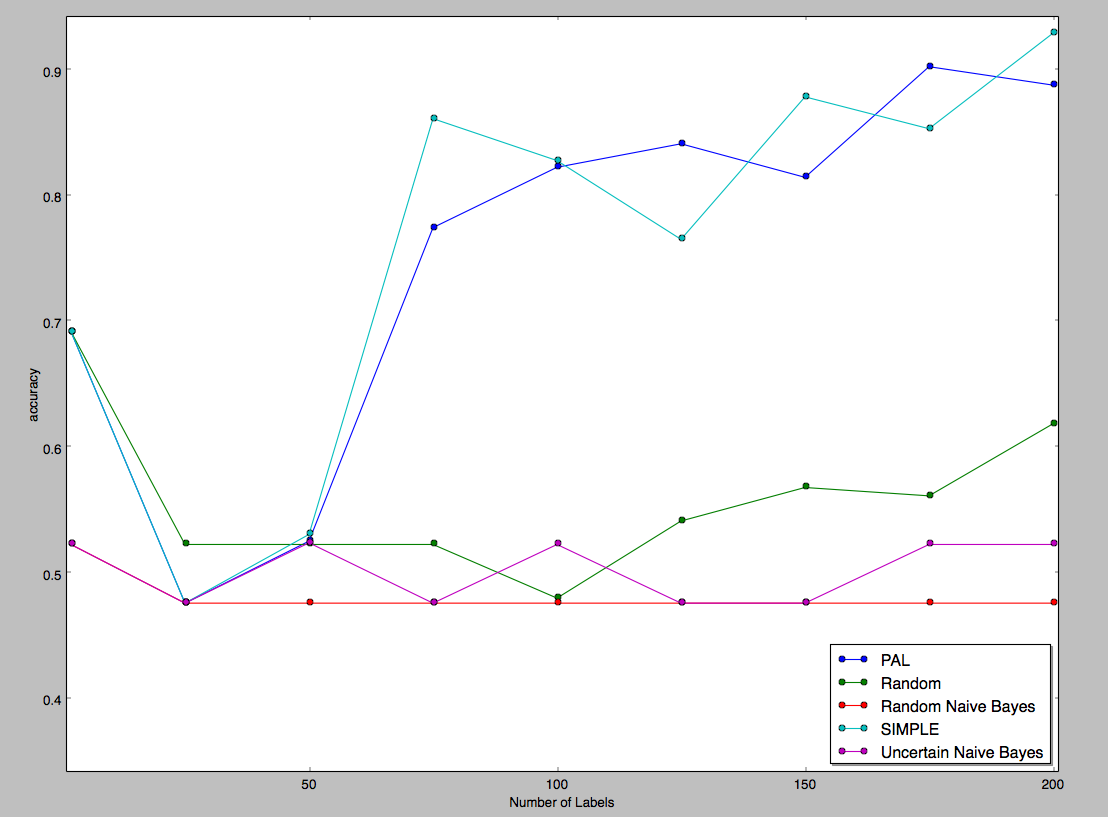
\includegraphics[scale=0.3]{activelearning/report}
  \caption{Active learning result}
 \end{figure}

As can be seen from the figure, if active sampling procedure is applied, the performance is on average better than random sampling method(the base test of the test). 


\item \textbf{Bayesian Nonparametric Model}
 \begin{itemize}
  \item Gained a general understanding of the theory
  \item Currently reviewing on the Gaussian process used for BNP regression
  \item Primary framework programming 
 \end{itemize}
 \end{itemize}
\section{Conclusion}

In this proposal, we concerned about the shortcoming in traditional active learning and bayesian nonparametric model in order to make them more applicable on big data problem. To adress these problems, we propose to introduce bayesian nonparametric model to active learning framework. On one hand, active learning theory is motivated on the scenario that concerns learning cost. It actively queries samples that will mostly improve the performance at each step, reaching similar or better performance than traditional supervised learning methods but at less cost.  On the other hand, BNP model tries to slove the constraints of parameters by combining the bayesian and non-parametric methods. It allows for a dynamic change of param- eters in the learning procedure. This flexibility is very important when trying to learn on ever-changing and complex data sets. As in big data set, abundancy and complexity are more likely to happen than on small data set. We aim to take advantages of the merits , as for active learning the efficiency and for BNP the flexibility, to make up for their disadvantage, as for active learning low sampling procedure and and for BNP low convergency rate, thus this whole framework will perform better both on efficiency and on accuracy in big dataset. 




%\bibliographystyle{amsplain} % By default (using th plain style) BibTeX orders citations alphabetically
%\bibliographystyle{bib_style} %references to be listed in the order of appeareance
%\addcontentsline{toc}{chapter}{Bibliography}
\addcontentsline{toc}{section}{Bibliography}
\bibliographystyle{abbrv} %references to be listed in the order of appeareance
%\bibliographystyle{bib_style}
%\newpage
\bibliography{refer}

\end{spacing}
\end{document}

